\documentclass[12pt,letterpaper]{article}

\usepackage[utf8]{inputenc}
\usepackage[T1]{fontenc}
\usepackage[spanish,es-tabla]{babel}
\usepackage{geometry}
\usepackage{graphicx}
\usepackage{float}
\usepackage{booktabs}
\usepackage{array}
\usepackage{hyperref}
\usepackage{tikz}
\usetikzlibrary{patterns,calc}
\usepackage{amsmath}

\geometry{margin=2.5cm}
\setlength{\parindent}{0pt}
\setlength{\parskip}{0.8em}

\hypersetup{
    colorlinks=true,
    linkcolor=black,
    urlcolor=black
}

\begin{document}
\shorthandoff{<>}

\pagenumbering{gobble}
\begin{titlepage}
    \centering
    \vspace*{1cm}

    {\Large \scshape Universidad Nacional de Colombia\par}
    \vspace{0.3cm}
    {\large \scshape Facultad de Minas\par}

    \vspace{0.5cm}
    \rule{\linewidth}{0.4pt}
    \vspace{1cm}

    {\Huge \textbf{Diseño preliminar de nervios de una losa de dos direcciones para una estructura de acero}\par}
    \vspace{0.6cm}

    \vspace{0.3cm}
    {\large Diseño Basico de Estructuras de Acero\par}

    \vspace{1cm}
    \rule{\linewidth}{0.4pt}

    \vfill

    {\bfseries Integrantes\par}
    \vspace{0.4cm}
    Juan Miguel Rojas Álvarez\par
    Miguel Ángel Medina Muñoz\par
    Jhon Alexander Hernandez Londoño\par

    \vspace{0.8cm}

    \textbf{Profesor:} \, Juan Fernando Velásquez Bedoya\par
    \vspace{0.3cm}
    \textbf{Fecha de entrega:} \, 25 de septiembre de 2026
\end{titlepage}

\pagenumbering{roman}
\tableofcontents
\newpage
\pagenumbering{arabic}

\section{Descripción general}

Este informe presenta el diseño preliminar de una losa maciza de concreto reforzado, abarcando desde el diseño arquitectonico del plano seleccionado, el calculo de cargas que debe soportar dos nervios en la misma dirección, tambien estimando una primera sección a partir del calculo de los diagramas de momentos.

\section{Planta estructural propuesta}

La planta estructural propuesta corresponde a una losa maciza de concreto reforzado con soporte en elementos de acero organizada sobre los ejes A-B-C-D y 1-2-3-4. La geometria general ocupa un rectangulo de 16,00 m por 16,00 m, con una modulacion horizontal de 8,00 m, 3,00 m y 5,00 m, y una modulacion vertical de 6,00 m, 5,00 m y 5,00 m. En el costado derecho central se conserva un vacio de 5,00 m por 5,00 m, destinado a la zona de escaleras del edificio.

El diseño arquitectonico se plantea con una franja central de corredor entre los ejes B y C, de 3,00 m de ancho, y con zonas de oficinas distribuidas a ambos lados, además se plantea en el espacio vacio ubicar la zona de escaleras.

\begin{figure}[H]
    \centering
    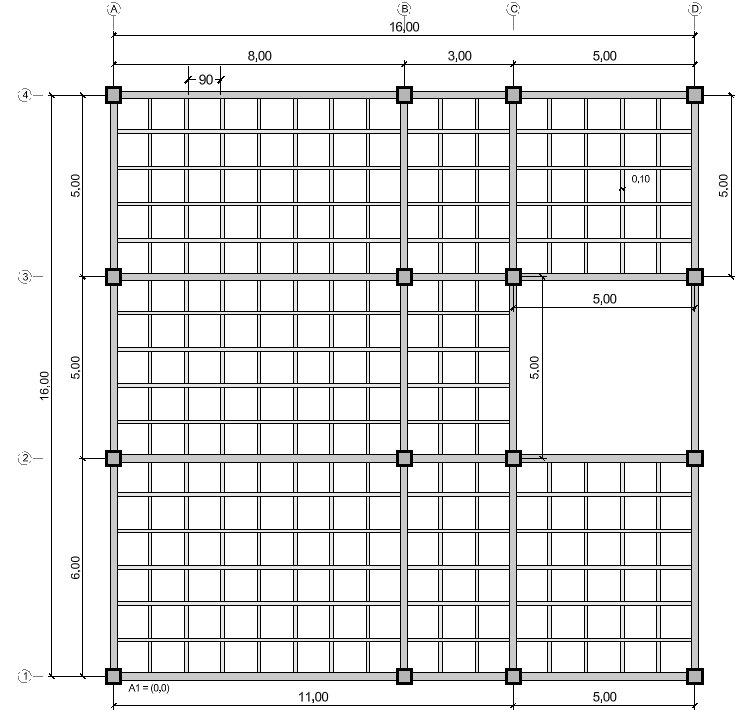
\includegraphics[width=0.65\textwidth]{../plano/Captura de pantalla 2026-09-15 125706.png}
    \caption{Planta estructural de losa maciza.}
    \label{fig:planta}
\end{figure}

\begin{figure}[H]
    \centering
    \begin{tikzpicture}[x=0.5cm, y=0.5cm, font=\small]
        % Zonas
        \fill[green!12] (0,0) rectangle (8,6);
        \fill[green!12] (0,6) rectangle (8,11);
        \fill[green!12] (0,11) rectangle (8,16);
        \fill[blue!10] (8,0) rectangle (11,16);
        \fill[green!12] (11,0) rectangle (16,6);
        \fill[green!12] (11,11) rectangle (16,16);
        \fill[gray!10] (11,6) rectangle (16,11);
        \foreach \yy in {6.5,7.0,...,10.5} {
            \draw[gray!65] (11.4,\yy) -- (15.6,\yy);
        }
        \draw[->, gray!70] (13.5,6.6) -- (13.5,10.4);

        % Ejes estructurales principales
        \draw[very thick] (0,0) -- (0,16);
        \draw[very thick] (8,0) -- (8,16);
        \draw[ultra thick] (11,0) -- (11,16);
        \draw[very thick] (16,0) -- (16,6);
        \draw[very thick] (16,11) -- (16,16);
        \draw[very thick] (0,0) -- (16,0);
        \draw[very thick] (0,16) -- (16,16);

        % Ejes internos discontinuos
        \draw[dashed, gray] (0,6) -- (8,6);
        \draw[dashed, gray] (0,11) -- (8,11);
        \draw[dashed, gray] (11,6) -- (16,6);
        \draw[dashed, gray] (11,11) -- (16,11);

        % Etiquetas de zona
        \node[align=center] at (4,3) {\textbf{OFICINA 1}\\8.00 $\times$ 6.00 m\\48 m\textsuperscript{2}};
        \node[align=center] at (4,8.5) {\textbf{OFICINA 2}\\8.00 $\times$ 5.00 m\\40 m\textsuperscript{2}};
        \node[align=center] at (4,13.5) {\textbf{OFICINA 3}\\8.00 $\times$ 5.00 m\\40 m\textsuperscript{2}};
        \node[align=center, text=blue!50!black, rotate=90] at (9.5,8) {\textbf{CORREDOR} -- 3.00 $\times$ 16.00 m};
        \node[align=center] at (13.5,3) {\textbf{OFICINA 4}\\5.00 $\times$ 6.00 m\\30 m\textsuperscript{2}};
        \node[align=center, text=gray!70!black, rotate=90] at (13.5,8.5) {\scriptsize\textbf{ESCALERAS}};
        \node[align=center] at (13.5,13.5) {\textbf{OFICINA 5}\\5.00 $\times$ 5.00 m\\25 m\textsuperscript{2}};

        % Etiquetas de ejes
        \node[above] at (0,16) {A};
        \node[above] at (8,16) {B};
        \node[above] at (11,16) {C};
        \node[above] at (16,16) {D};
        \node[left] at (0,0) {1};
        \node[left] at (0,6) {2};
        \node[left] at (0,11) {3};
        \node[left] at (0,16) {4};

        % Cotas horizontales
        \draw[<->] (0,-1) -- (8,-1) node[midway, below] {8.00};
        \draw[<->] (8,-1) -- (11,-1) node[midway, below] {3.00};
        \draw[<->] (11,-1) -- (16,-1) node[midway, below] {5.00};

        % Cotas verticales
        \draw[<->] (-1.4,0) -- (-1.4,6) node[midway, sloped, above] {6.00};
        \draw[<->] (-1.4,6) -- (-1.4,11) node[midway, sloped, above] {5.00};
        \draw[<->] (-1.4,11) -- (-1.4,16) node[midway, sloped, above] {5.00};
    \end{tikzpicture}
    \caption{Distribucion arquitectonica en planta.}
    \label{fig:distribucion}
\end{figure}

Por otro lado, se optó por una losa maciza de concreto reforzado de 0,05 m de espesor. Esto valor encontrado a partir de las formulas de prediseño otorgadas por la NSR-10, con la ecuación de L/20 dada por la tabla C.9.5.3.

\begin{figure}[H]
    \centering
    \begin{tikzpicture}[x=8cm, y=18cm, font=\small]
        \fill[gray!18] (0,0) rectangle (1,0.05);
        \draw[very thick] (0,0) rectangle (1,0.05);
        \draw[<->] (1.08,0) -- (1.08,0.05) node[midway, right] {$h = 0{,}05$ m};
        \draw[<->] (0,-0.025) -- (1,-0.025) node[midway, below] {$1{,}00$ m};
        \node at (0.5,0.025) {losa maciza de concreto reforzado};
    \end{tikzpicture}
    \caption{Modulo representativo por metro cuadrado de losa maciza.}
    \label{fig:modulo-nervio}
\end{figure}

Por ultimo cabe mencionar que la resistencia de compresion del concreto adoptada fue de 21 MPa y la resistencia de fluencia del acero usado fue de 420 MPa.
\section{Criterios iniciales de carga}
\label{sec:cargas}

Para el cálculo preliminar de cargas se tomó como referencia la NSR-10. A partir de la Tabla B.3.4.3-1, correspondiente a valores mínimos alternativos de carga muerta de elementos no estructurales cuando no se efectúa un análisis más detallado.

De acuerdo con la referencia marcada para ocupación de oficinas, se adoptan inicialmente los siguientes valores:

\begin{table}[H]
    \centering
    \begin{tabular}{>{\raggedright\arraybackslash}p{7cm} c}
        \toprule
        Concepto & Carga adoptada \\
        \midrule
        Particiones & 2,0 kN/m\textsuperscript{2} \\
        Acabados de piso y cubierta & 1,8 kN/m\textsuperscript{2} \\
        Instalaciones & 0,5 kN/m\textsuperscript{2} \\
        \bottomrule
    \end{tabular}
    \caption{Valores preliminares de carga muerta considerados.}
    \label{tab:cargas}
\end{table}

Para la carga viva se empleó la Tabla B.4.2.1-1, Cargas vivas mínimas uniformemente distribuidas.

\begin{table}[H]
    \centering
    \begin{tabular}{>{\raggedright\arraybackslash}p{7cm} c}
        \toprule
        Ocupación o uso & Carga viva \\
        \midrule
        Oficinas (zonas 1 a 5) & 2,0 kN/m\textsuperscript{2} \\
        Corredores (franja B-C) & 3,0 kN/m\textsuperscript{2} \\
        \bottomrule
    \end{tabular}
    \caption{Cargas vivas adoptadas según NSR-10, Tabla B.4.2.1-1.}
    \label{tab:cargas-vivas}
\end{table}

\subsection{Peso propio de la losa maciza}

Para este primer informe unicamente se toma la carga muerta de la losa maciza. El espesor adoptado es $h = 0{,}05$ m, por lo que el volumen unitario por metro cuadrado es:

\begin{equation}
v = 1{,}00 \cdot 1{,}00 \cdot 0{,}05 = 0{,}05 \ \text{m}^3/\text{m}^2
\end{equation}

Suponiendo un peso específico del concreto reforzado de $24$ kN/m\textsuperscript{3}, el peso propio de la losa resulta:

\begin{equation}
w_{pp} = 0{,}05 \ \text{m}^3/\text{m}^2 \times 24 \ \text{kN/m}^3 = 1{,}20 \ \text{kN/m}^2
\end{equation}

Este valor se suma a las cargas muertas del Cuadro \ref{tab:cargas} para obtener la carga muerta total de diseño:

\begin{table}[H]
    \centering
    \begin{tabular}{>{\raggedright\arraybackslash}p{7cm} c}
        \toprule
        Concepto & Carga \\
        \midrule
        Particiones & 2,0 kN/m\textsuperscript{2} \\
        Acabados de piso y cubierta & 1,8 kN/m\textsuperscript{2} \\
        Instalaciones & 0,5 kN/m\textsuperscript{2} \\
        Peso propio de la losa maciza & 1,20 kN/m\textsuperscript{2} \\
        \midrule
        \textbf{Carga muerta total (D)} & \textbf{5,50 kN/m\textsuperscript{2}} \\
        \bottomrule
    \end{tabular}
    \caption{Carga muerta total de diseño, incluyendo el peso propio calculado.}
    \label{tab:carga-muerta-total}
\end{table}

\subsection{Combinación de cargas mayoradas}

Con la carga muerta total $D = 5{,}50$ kN/m\textsuperscript{2} y las cargas vivas $L$ del Cuadro \ref{tab:cargas-vivas}, se calculó la carga última mediante la combinación $U = 1{,}2D + 1{,}6L$, considerando los dos usos de la planta:

\begin{align*}
U_{\text{oficinas}} &= 1{,}2(1{,}20+2+1{,}8+0{,}5) + 1{,}6(2) = 9{,}80 \ \text{kN/m}^2 \approx 10 \ \text{kN/m}^2 \\
U_{\text{corredores}} &= 1{,}2(1{,}20+2+1{,}8+0{,}5) + 1{,}6(3) = 11{,}40 \ \text{kN/m}^2 \approx 12 \ \text{kN/m}^2
\end{align*}

\begin{table}[H]
    \centering
    \begin{tabular}{>{\raggedright\arraybackslash}p{7cm} c}
        \toprule
        Zona & Carga última $U$ \\
        \midrule
        Oficinas (zonas 1 a 5) & 10 kN/m\textsuperscript{2} \\
        Corredor (franja B-C) & 12 kN/m\textsuperscript{2} \\
        \bottomrule
    \end{tabular}
    \caption{Cargas últimas de diseño por zona.}
    \label{tab:carga-ultima}
\end{table}

Estos valores de carga última son los que se emplearán como punto de partida para el diseño a flexión y cortante de la franja de losa analizada.

\section{Análisis de la franja continua por pendiente-deflexión a mano}
\label{sec:pendiente-deflexion}

Por otro lado, se analizarón dos nervios en la misma dirección con diferente espaciamiento entre los apoyos, estos nervios se pueden evidenciar en la figura 4.
\subsection{Esquema estructural y cargas}

La carga lineal sobre la franja se obtuvo multiplicando la carga última por metro cuadrado (Cuadro \ref{tab:carga-ultima}) por el ancho tributario correspondiente a cada tramo. No se adoptó un único factor para toda la franja, porque el tramo del corredor y los tramos de oficinas no reciben la misma franja tributaria de losa.

\begin{figure}[H]
    \centering
    \begin{tikzpicture}
        \node[anchor=south west,inner sep=0] (planta) at (0,0)
            {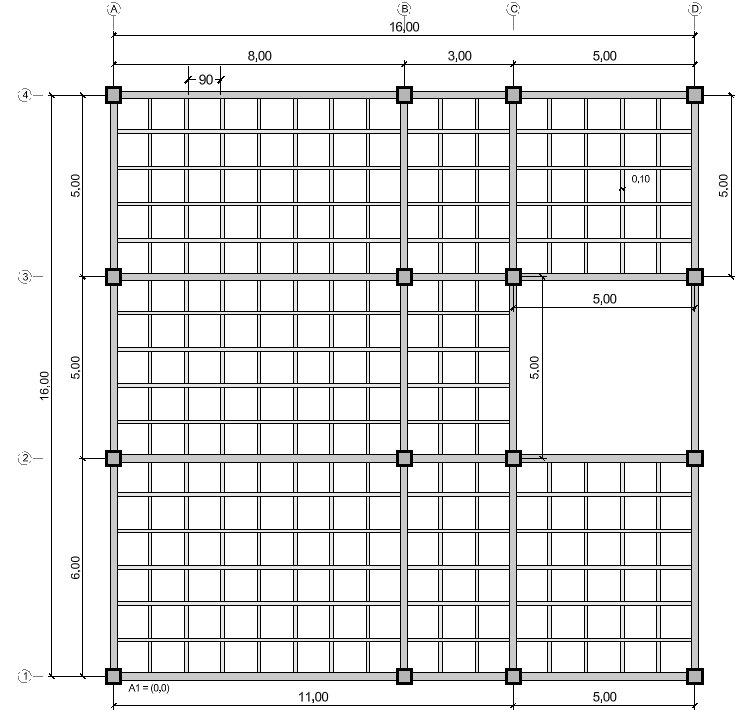
\includegraphics[width=0.92\textwidth]{../plano/Captura de pantalla 2026-09-15 125706.png}};
        \path (planta.south west) -- (planta.south east) coordinate[pos=0.151] (xA);
        \path (planta.south west) -- (planta.south east) coordinate[pos=0.685] (xC);
        \path (planta.south west) -- (planta.south east) coordinate[pos=0.925] (xD);
        \path (planta.south west) -- (planta.north west) coordinate[pos=0.814] (yN1);
        \path (planta.south west) -- (planta.north west) coordinate[pos=0.578] (yN2);
        \draw[red!80!black,line width=3pt,opacity=0.82] (xA |- yN1) -- (xD |- yN1);
        \draw[orange!90!black,line width=3pt,opacity=0.88] (xA |- yN2) -- (xC |- yN2);
        \path (xA |- yN1) -- (xD |- yN1) coordinate[pos=0.34] (tagN1);
        \path (xA |- yN2) -- (xC |- yN2) coordinate[pos=0.30] (tagN2);
        \node[above,fill=white,inner sep=1pt,text=red!80!black,font=\scriptsize\bfseries] at (tagN1) {Nervio 1};
        \node[above,fill=white,inner sep=1pt,text=orange!75!black,font=\scriptsize\bfseries] at (tagN2) {Nervio 2};
    \end{tikzpicture}
    \caption{Ubicación en planta de los nervios analizados.}
    \label{fig:planta-nervio-analizado}
\end{figure}

\begin{align*}
w_1 &= 10 \times 0{,}40 = 4{,}00 \ \text{kN/m} \quad \text{(A-B, oficina)} \\
w_2 &= 12 \times 0{,}60 = 7{,}20 \ \text{kN/m} \quad \text{(B-C, corredor)} \\
w_3 &= 10 \times 0{,}50 = 5{,}00 \ \text{kN/m} \quad \text{(C-D, oficina)}
\end{align*}

\begin{figure}[H]
    \centering
    \begin{tikzpicture}[x=0.55cm, y=0.5cm, font=\footnotesize]
        % Beam line
        \draw[very thick] (0,0) -- (16,0);
        % Supports (triangles)
        \foreach \x in {0,8,11,16} {
            \draw (\x,0) -- (\x-0.4,-0.9) -- (\x+0.4,-0.9) -- cycle;
            \draw[fill=black] (\x,0) circle (0.05);
        }
        % Load arrows spans 1 and 3 (lower)
        \foreach \x in {0.5,1.5,...,7.5} {\draw[->] (\x,1.0) -- (\x,0.05);}
        \foreach \x in {11.5,12.5,...,15.5} {\draw[->] (\x,1.0) -- (\x,0.05);}
        \draw (0,1.0) -- (8,1.0);
        \draw (11,1.0) -- (16,1.0);
        % Load arrows span 2 (higher, corredor)
        \foreach \x in {8.5,9.5,10.5} {\draw[->] (\x,1.7) -- (\x,0.05);}
        \draw (8,1.7) -- (11,1.7);
        % Load labels
        \node[above] at (4,1.0) {$w_1 = 4{,}00$ kN/m};
        \node[above] at (9.5,1.7) {$w_2 = 7{,}20$ kN/m};
        \node[above] at (13.5,1.0) {$w_3 = 5{,}00$ kN/m};
        % Joint labels
        \node[below] at (0,-0.9) {A};
        \node[below] at (8,-0.9) {B};
        \node[below] at (11,-0.9) {C};
        \node[below] at (16,-0.9) {D};
        % Span dimension labels
        \node[below] at (4,-2.3) {$L_1 = 8$ m};
        \node[below] at (9.5,-2.3) {$L_2 = 3$ m};
        \node[below] at (13.5,-2.3) {$L_3 = 5$ m};
    \end{tikzpicture}
    \caption{Esquema de la franja continua analizada.}
    \label{fig:esquema-nervio}
\end{figure}

\subsection{Momentos de empotramiento}

Aplicando los terminos de pendiente deflexión sobre los tramos quedan las siguientes expresiones:

\begin{align*}
\text{Tramo 1 (extremo A articulado):} \quad & \frac{3EI}{L_1} = \frac{3EI}{8} \\
\text{Tramo 2 (extremo B, cercano):} \quad & \frac{4EI}{L_2} = \frac{4EI}{3} \qquad \text{(extremo C, transporte)} \quad \frac{2EI}{L_2} = \frac{2EI}{3} \\
\text{Tramo 3 (extremo D articulado):} \quad & \frac{3EI}{L_3} = \frac{3EI}{5}
\end{align*}

Los momentos de empotramiento o momentos generados por las cargas externas (FEM) se calculan con la fórmula reducida $wL^2/8$ para los tramos con extremos articulados, y con la fórmula estándar $wL^2/12$ para el tramo interior con empotramientos:

\begin{align*}
\text{FEM}_1 = \frac{w_1 L_1^2}{8} = \frac{4{,}00 \times 8^2}{8} &= 32{,}00 \ \text{kN·m} \\
\text{FEM}_2 = \frac{w_2 L_2^2}{12} = \frac{7{,}20 \times 3^2}{12} &= 5{,}40 \ \text{kN·m} \\
\text{FEM}_3 = \frac{w_3 L_3^2}{8} = \frac{5{,}00 \times 5^2}{8} &= 15{,}63 \ \text{kN·m}
\end{align*}

\subsection{Ecuaciones de equilibrio y solución}

Planteando el equilibrio de momentos en cada nudo interior ($M_{BA}+M_{BC}=0$ en B, $M_{CB}+M_{CD}=0$ en C) y con los diagramas guias que se enseño en clase queda la siguientes expresiones:

\begin{align*}
\text{Nudo B:} \quad &\left(\frac{3EI}{8}+\frac{4EI}{3}\right)\theta_2 + \frac{2EI}{3}\theta_3 + \text{FEM}_2 - \text{FEM}_1 = 0 \\
\text{Nudo C:} \quad &\frac{2EI}{3}\theta_2 + \left(\frac{4EI}{3}+\frac{3EI}{5}\right)\theta_3 + \text{FEM}_3 - \text{FEM}_2 = 0
\end{align*}

\begin{figure}[H]
    \centering
    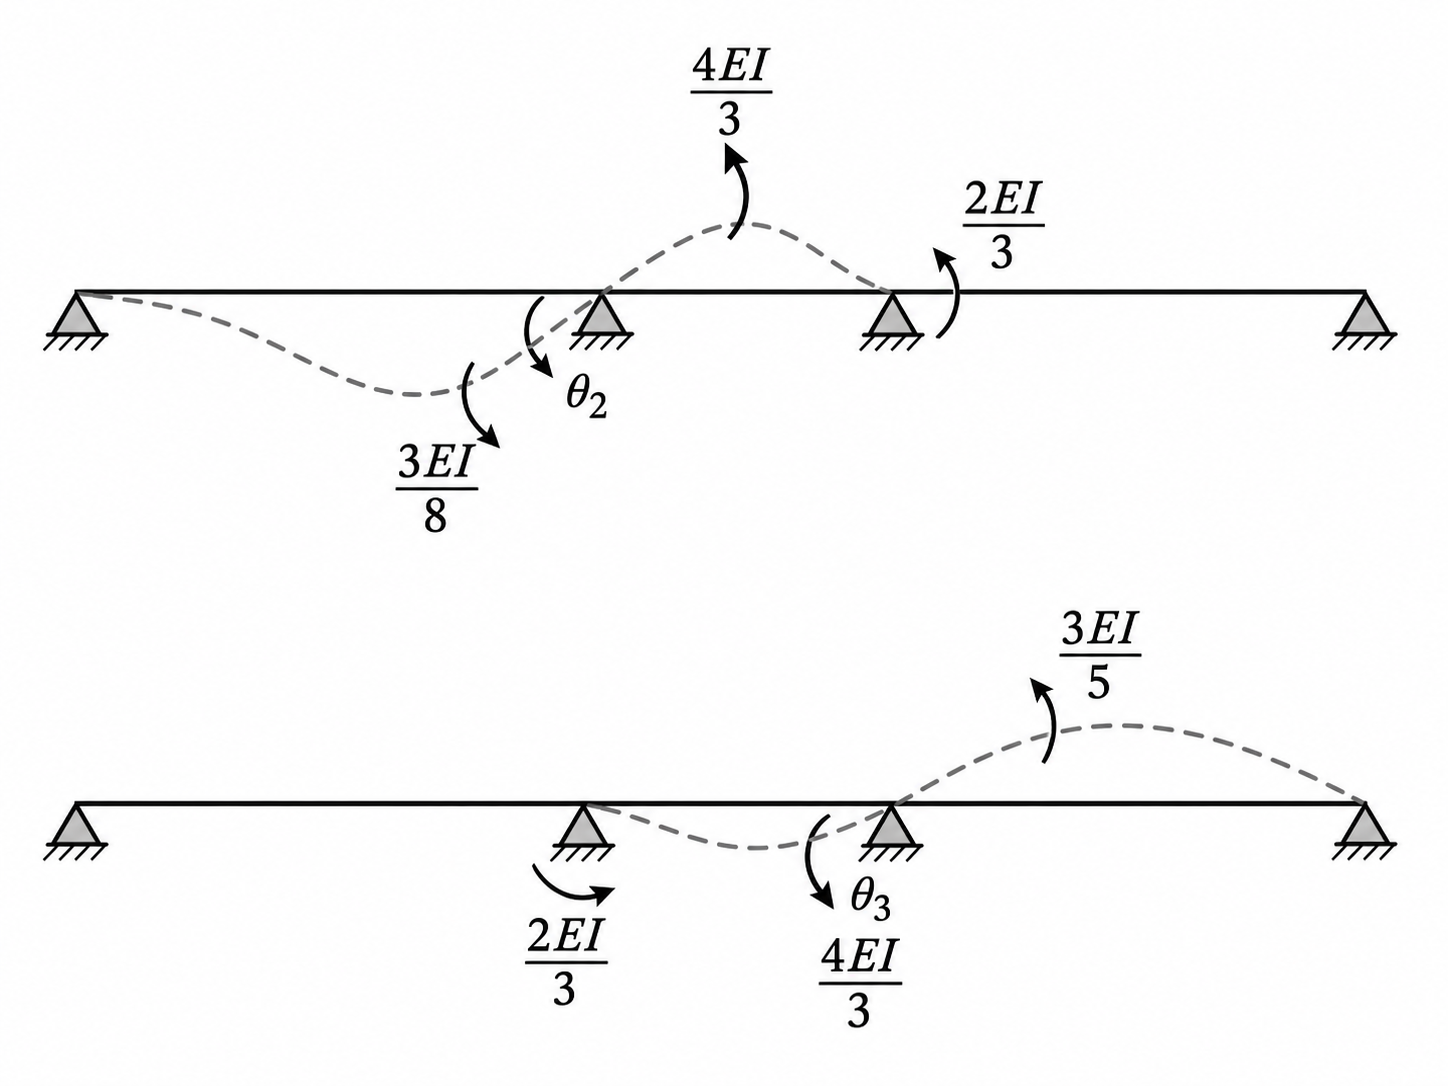
\includegraphics[width=0.78\textwidth]{figuras/continuidad_pendiente_deflexion.png}
    \caption{Esquema guia para las ecuaciones de continuidad en los nudos B y C.}
    \label{fig:continuidad-pendiente-deflexion}
\end{figure}

lo que conduce al sistema matricial (con $\Theta = EI\theta$):

\begin{equation}
\begin{bmatrix} \dfrac{41}{24} & \dfrac{2}{3} \\[2mm] \dfrac{2}{3} & \dfrac{29}{15} \end{bmatrix}
\begin{bmatrix} \Theta_2 \\ \Theta_3 \end{bmatrix}
=
\begin{bmatrix} \text{FEM}_1 - \text{FEM}_2 \\ \text{FEM}_2 - \text{FEM}_3 \end{bmatrix}
=
\begin{bmatrix} 26{,}60 \\ -10{,}23 \end{bmatrix}
\end{equation}

Resolviendo el sistema:

\begin{equation}
\theta_2 = \frac{20{,}377}{EI} \qquad \theta_3 = \frac{-12{,}290}{EI}
\end{equation}

\subsection{Momentos en los apoyos}

Con $\theta_2$ y $\theta_3$ ya conocidos, los momentos en cada extremo de tramo se obtienen de las mismas ecuaciones de pendiente-deflexión, evaluando $\Theta_2 = EI\theta_2 = 20{,}377$ y $\Theta_3 = EI\theta_3 = -12{,}290$ quedando las siguientes expresiones:

\begin{align*}
M_{BA} &= \frac{3}{8}\Theta_2 - \text{FEM}_1 = \frac{3}{8}(20{,}377) - 32{,}00 = -24{,}36 \ \text{kN·m} \\
M_{CB} &= \frac{2}{3}\Theta_2 + \frac{4}{3}\Theta_3 - \text{FEM}_2 = \frac{2}{3}(20{,}377) + \frac{4}{3}(-12{,}290) - 5{,}40 = -8{,}24 \ \text{kN·m}
\end{align*}

Resumiendo los momentos en la siguiente tabla queda: 

\begin{table}[H]
    \centering
    \begin{tabular}{>{\raggedright\arraybackslash}p{6cm} c}
        \toprule
        Apoyo & Momento \\
        \midrule
        $M_2$ (apoyo B) & $-24{,}36$ kN·m \\
        $M_3$ (apoyo C) & $-8{,}24$ kN·m \\
        \bottomrule
    \end{tabular}
    \caption{Momentos finales en los apoyos intermedios de la franja continua analizada.}
    \label{tab:momentos-nervio}
\end{table}

Estos momentos sirven como referencia para la elección de la sección de acero para los nervios. El segundo nervio se analiza con Xvigas en la Sección \ref{sec:nervio2-xvigas}, y ambos resultados se consideran para la preselección del perfil de acero.

\subsection{Reacciones, y diagramas de cortante y de momento}

Con los momentos de apoyo ya conocidos, las reacciones se calcularon por equilibrio estático en cada tramo

\begin{align*}
R_{B1} &= \frac{w_1L_1^2/2 - M_B}{L_1} = 19{,}04 \ \text{kN}
&
R_{A1} &= w_1L_1 - R_{B1} = 12{,}96 \ \text{kN} \\
R_{B2} &= \frac{w_2L_2^2/2 + M_B - M_C}{L_2} = 5{,}43 \ \text{kN}
&
R_{A2} &= w_2L_2 - R_{B2} = 16{,}17 \ \text{kN} \\
R_{B3} &= \frac{w_3L_3^2/2 + M_C}{L_3} = 10{,}85 \ \text{kN}
&
R_{A3} &= w_3L_3 - R_{B3} = 14{,}15 \ \text{kN}
\end{align*}

Las reacciones en los apoyos globales se obtienen sumando las contribuciones de los tramos que llegan a cada nudo:

\begin{table}[H]
    \centering
    \begin{tabular}{>{\raggedright\arraybackslash}p{6cm} c}
        \toprule
        Apoyo & Reacción \\
        \midrule
        $R_A=R_{A1}$ & $12{,}96$ kN \\
        $R_B=R_{B1}+R_{A2}$ & $35{,}22$ kN \\
        $R_C=R_{B2}+R_{A3}$ & $19{,}57$ kN \\
        $R_D=R_{B3}$ & $10{,}85$ kN \\
        \midrule
        \textbf{Suma} $\sum R_i$ & \textbf{78{,}60 kN} \\
        \bottomrule
    \end{tabular}
    \caption{Reacciones de la franja continua.}
    \label{tab:reacciones-nervio}
\end{table}

Después de definir las reacciones, se construyen las funciones de cortante y momento para graficar los diagramas. En coordenada global $x$, las funciones empleadas son:

\begin{align*}
V_1(x) &= R_{A1}-w_1x && 0 \leq x \leq 8 \\
V_2(x) &= R_{A2}-w_2(x-8) && 8 \leq x \leq 11 \\
V_3(x) &= R_{A3}-w_3(x-11) && 11 \leq x \leq 16 \\
M_1(x) &= R_{A1}x-\frac{w_1x^2}{2} && 0 \leq x \leq 8 \\
M_2(x) &= M_B+R_{A2}(x-8)-\frac{w_2(x-8)^2}{2} && 8 \leq x \leq 11 \\
M_3(x) &= M_C+R_{A3}(x-11)-\frac{w_3(x-11)^2}{2} && 11 \leq x \leq 16
\end{align*}

Con estas expresiones se obtienen los diagramas de fuerza cortante y de momento flector del nervio seleccionado (Figura \ref{fig:dfc-dmf}). Los momentos positivos principales ocurren en la Oficina 1 ($+20{,}98$ kN·m, a $3{,}24$ m de A) y en la Oficina 4 ($+11{,}78$ kN·m, a $2{,}83$ m de C).

\begin{figure}[H]
    \centering
    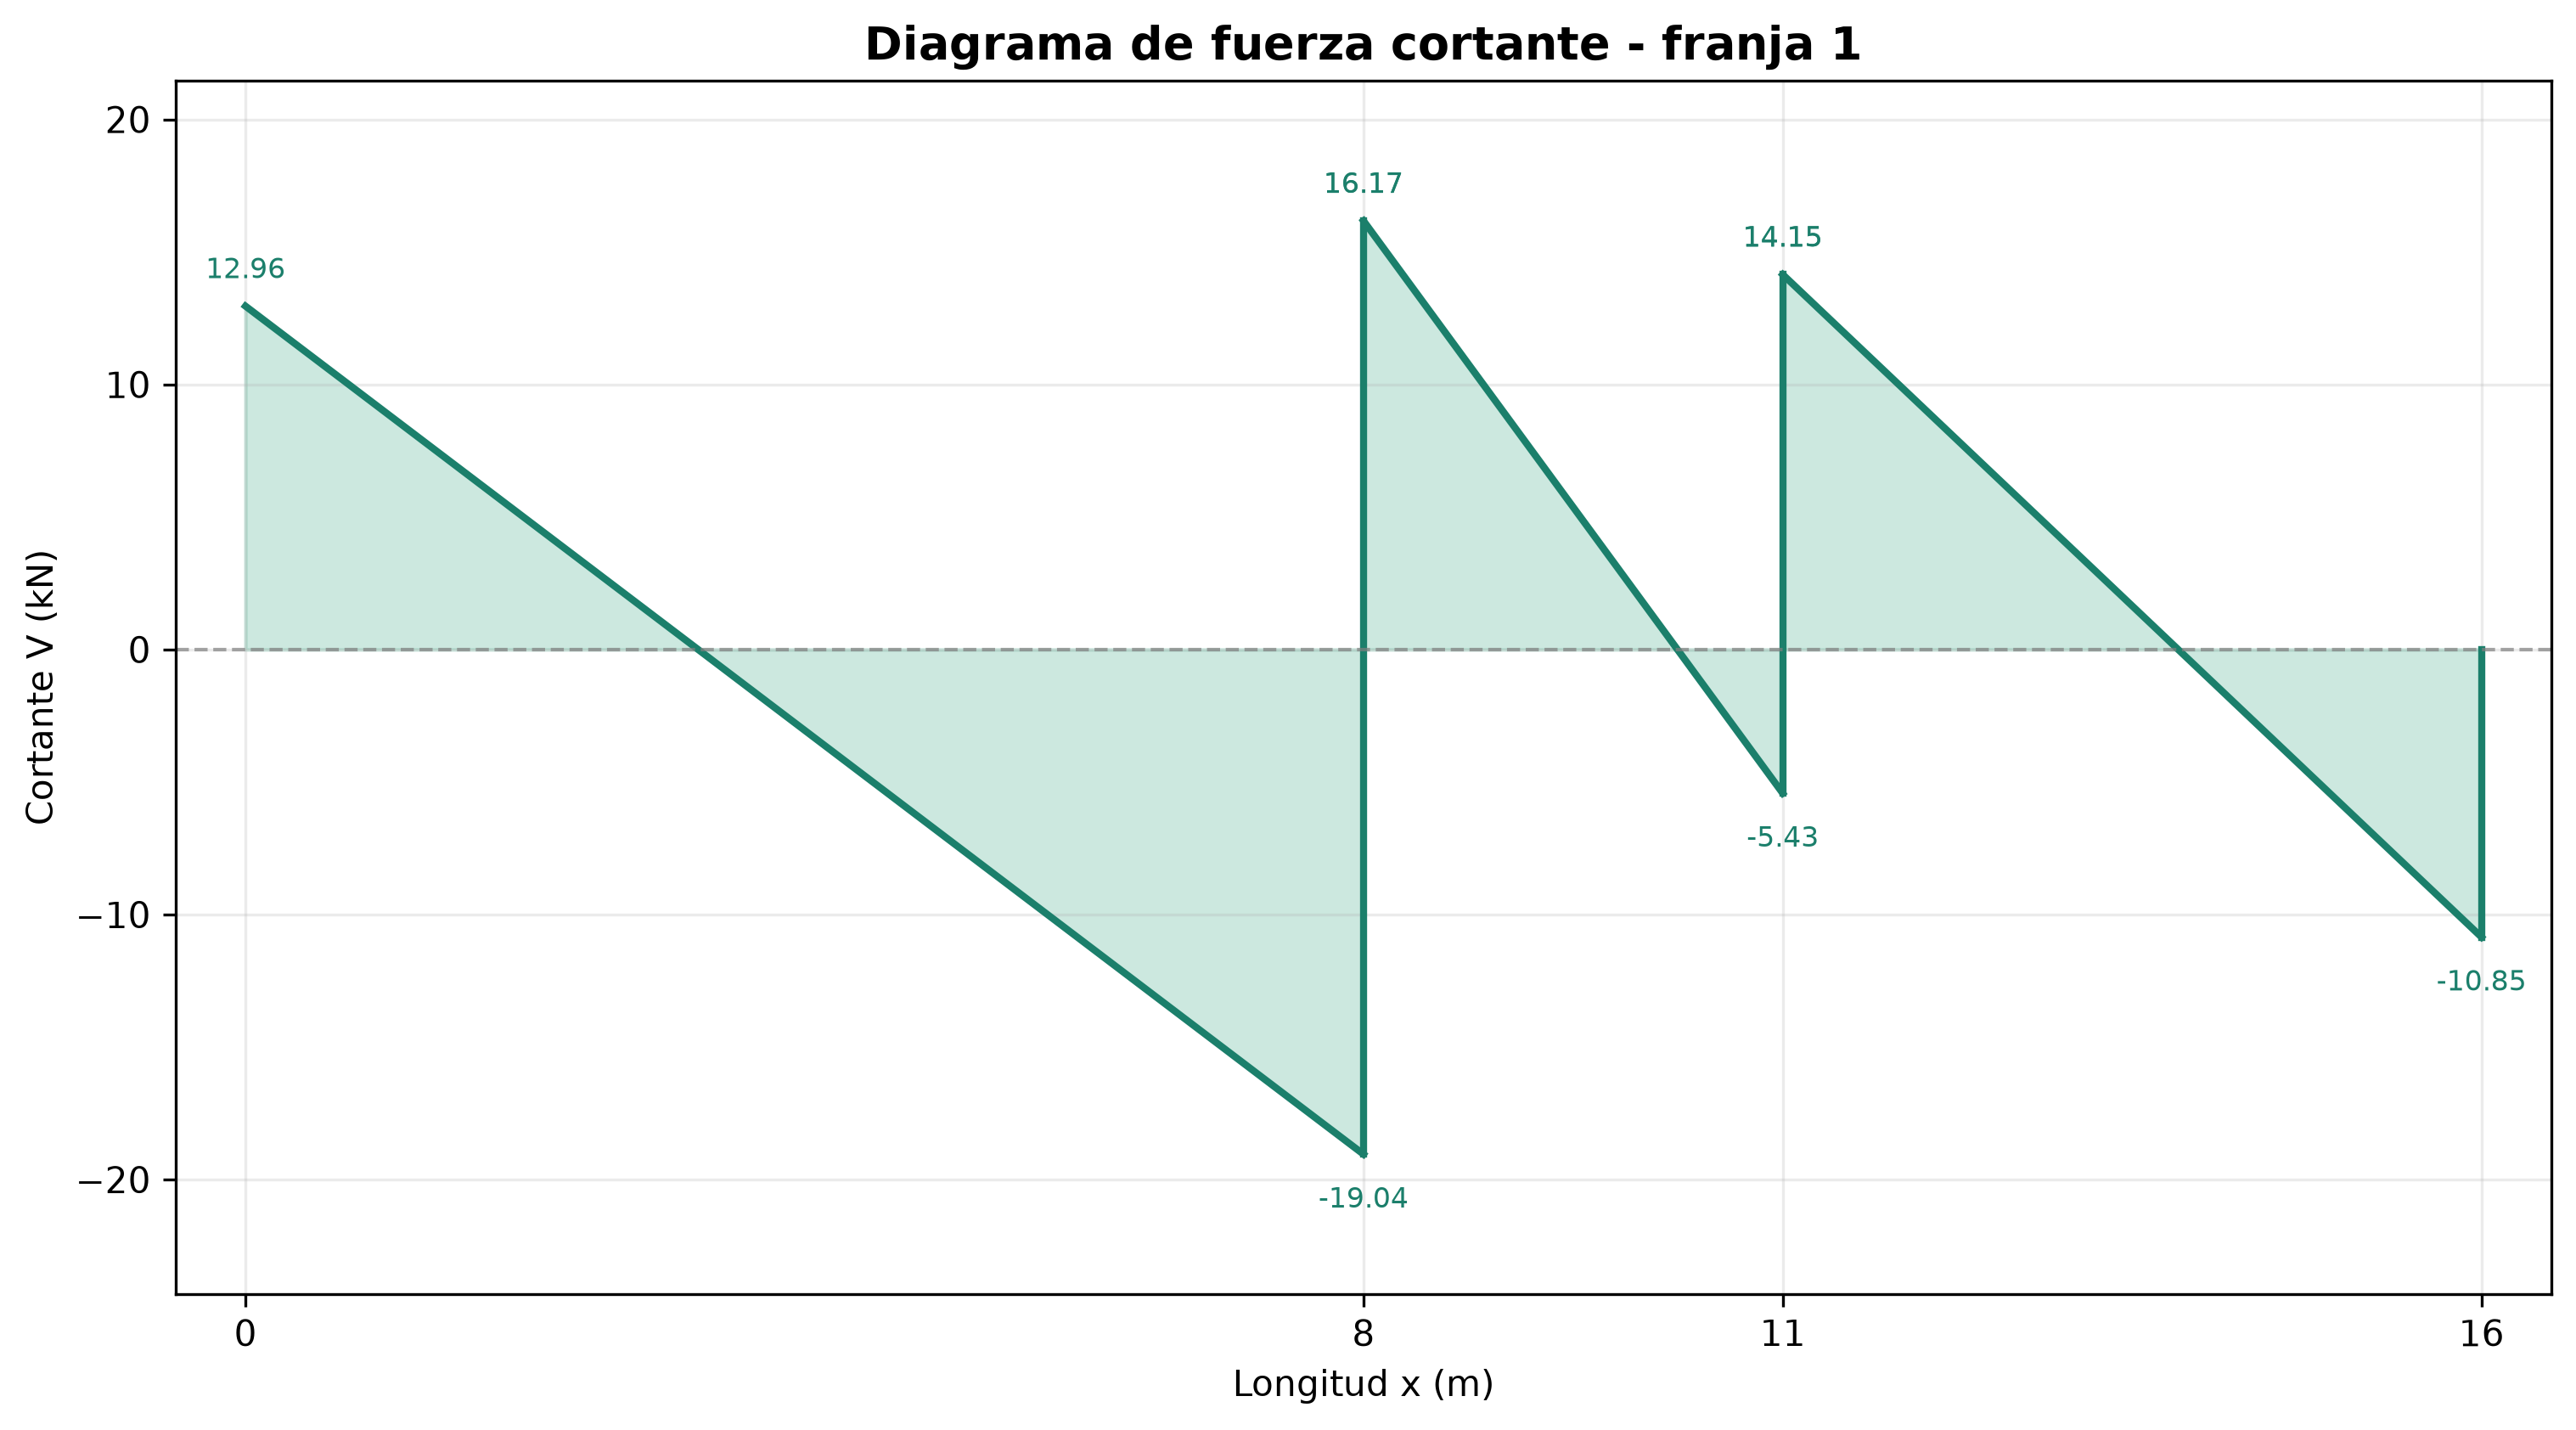
\includegraphics[width=0.92\textwidth]{figuras/diagrama_cortante_nervio1.png}
    \vspace{0.4cm}

    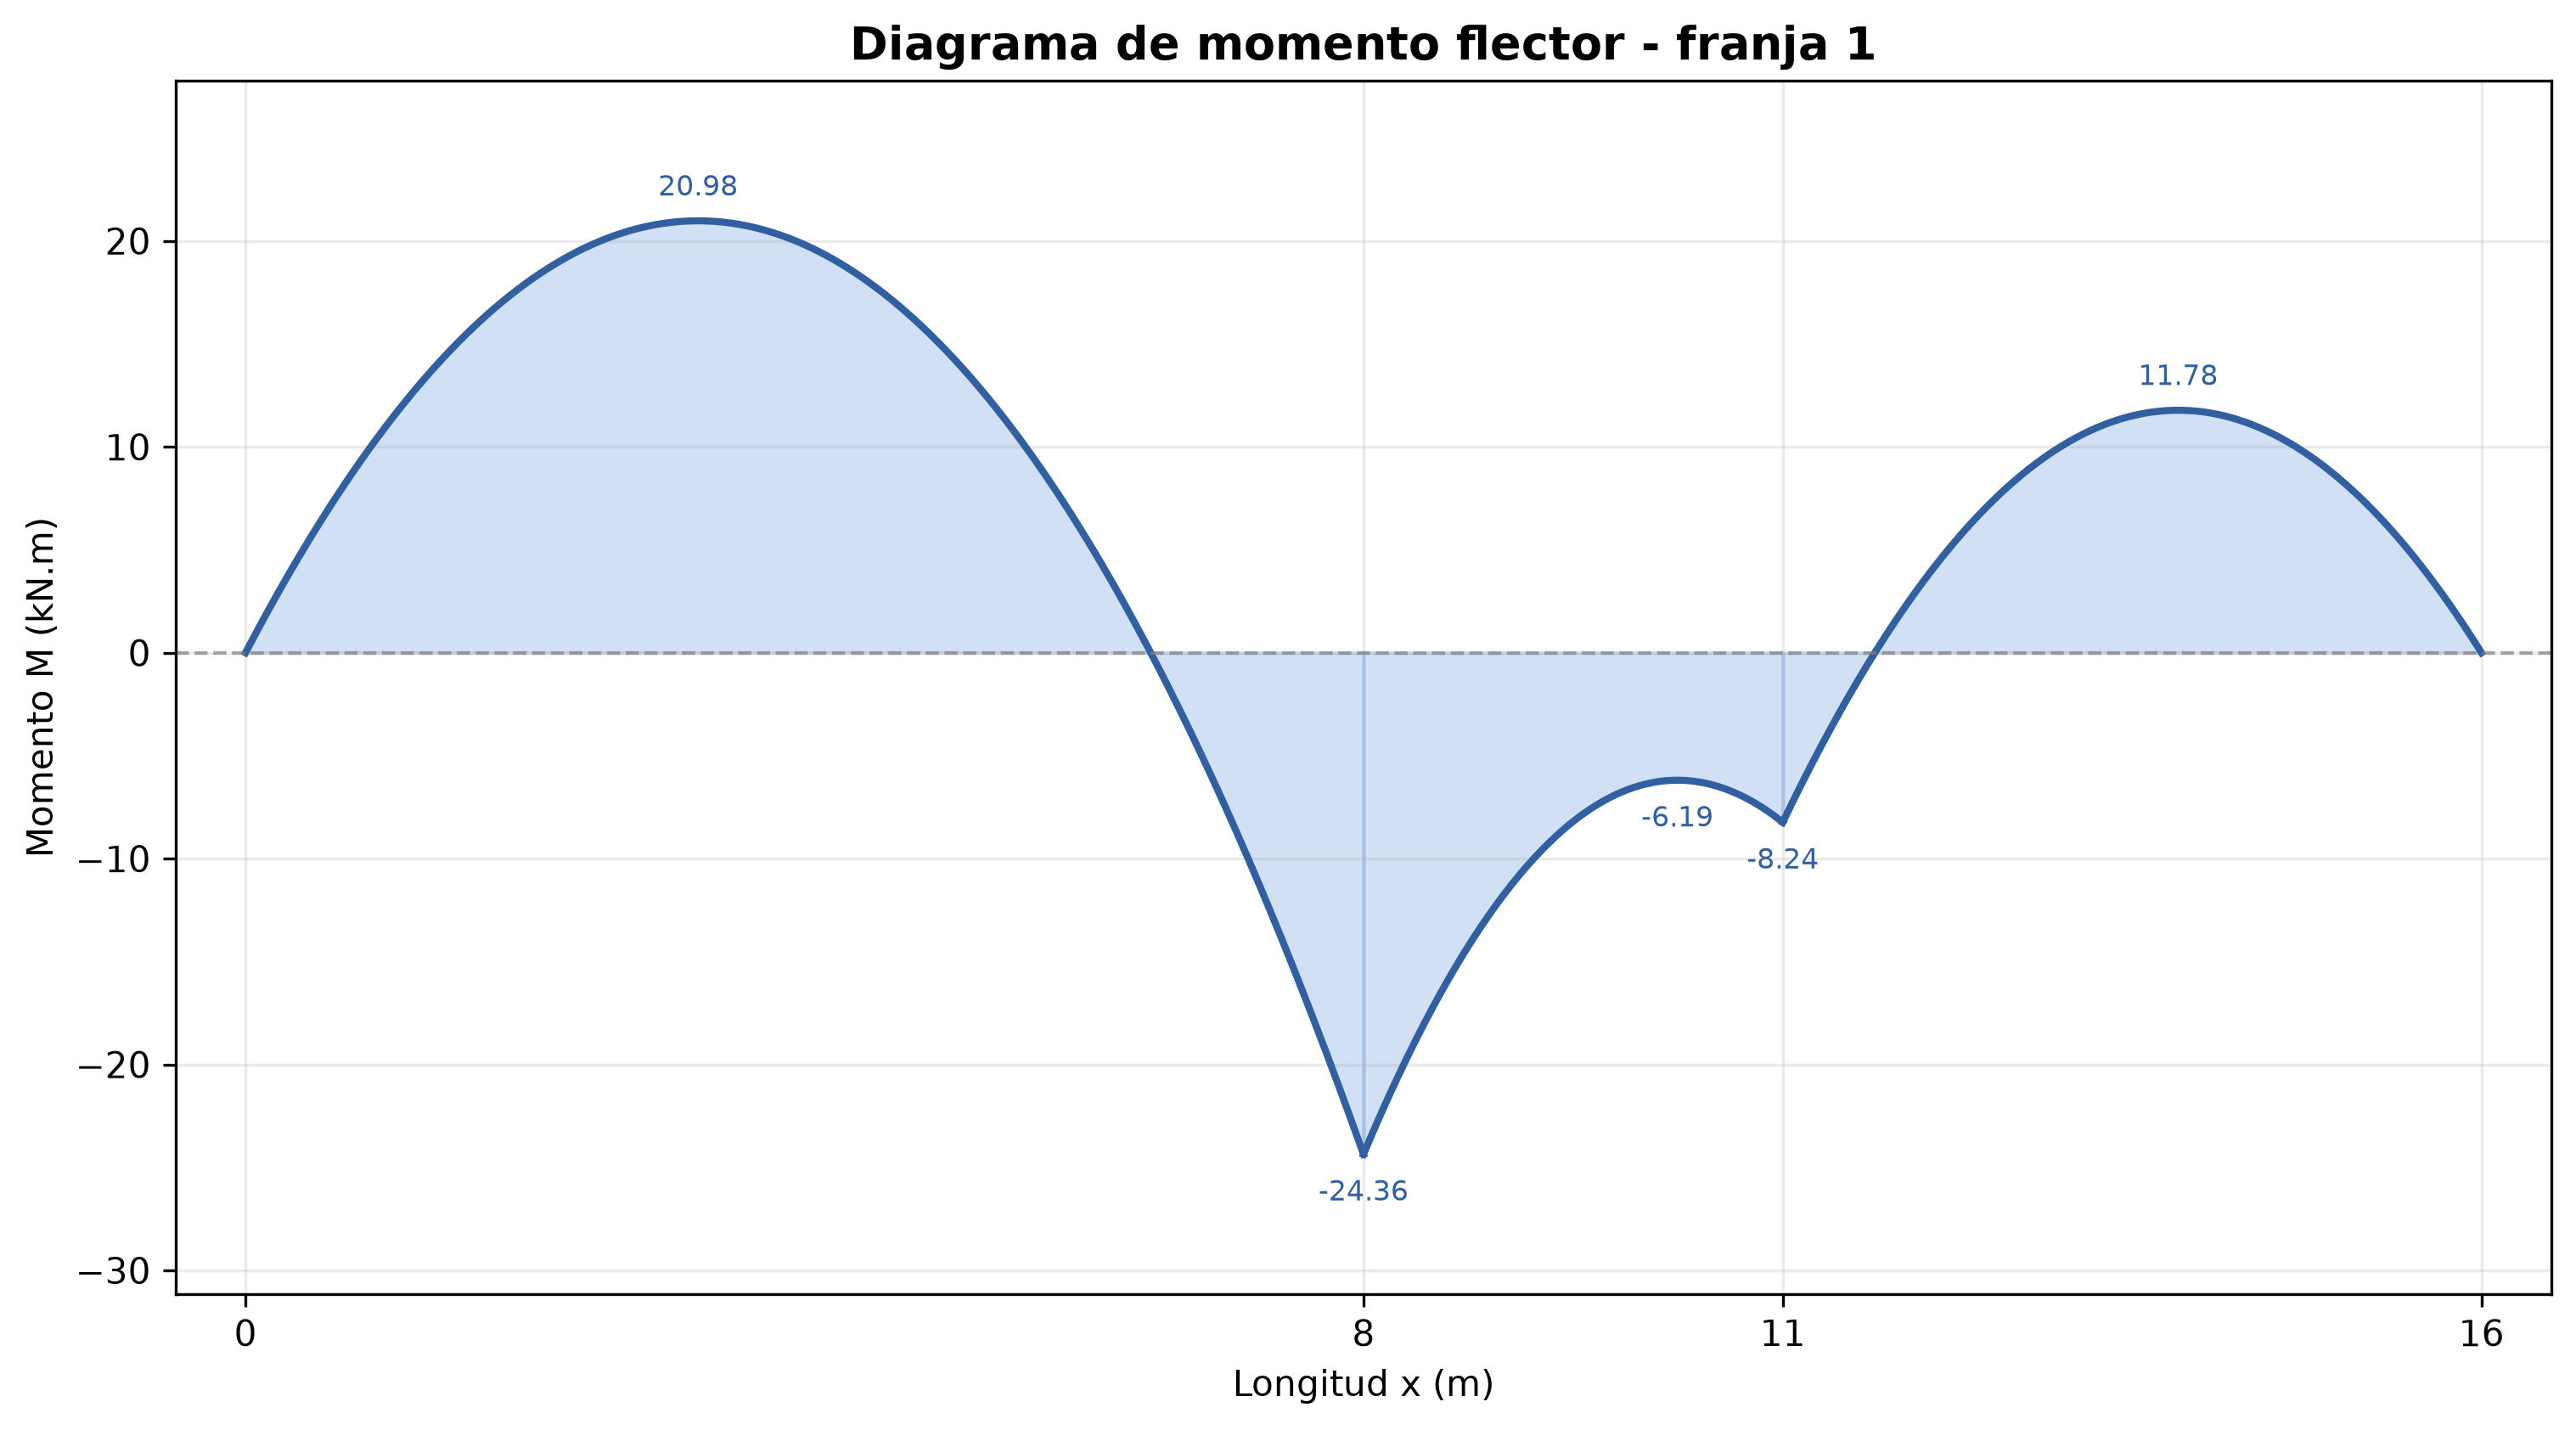
\includegraphics[width=0.92\textwidth]{figuras/diagrama_momento_nervio1.png}
    \caption{Diagrama de fuerza cortante (DFC, kN) y diagrama de momento flector (DMF, kN·m) de la franja analizada a mano.}
    \label{fig:dfc-dmf}
\end{figure}

\section{Análisis del segundo nervio con Xvigas}
\label{sec:nervio2-xvigas}

Se analizó además el primer nervio horizontal superior de la Oficina 2, continuo hacia el corredor entre los ejes A y C. El modelo de Xvigas comprende dos tramos: A-B de 8,00 m, cargado con $4,00$ kN/m, y B-C de 3,00 m, cargado con $7,20$ kN/m.

La Figura \ref{fig:xvigas-cargas} muestra el modelo y las cargas introducidas. Los diagramas de cortante y momento de las Figuras \ref{fig:xvigas-cortante} y \ref{fig:xvigas-momento} se incorporan directamente desde los resultados de Xvigas. El momento negativo en B es aproximadamente $-25{,}52$ kN·m y el momento positivo máximo en el tramo A-B es aproximadamente $+20{,}51$ kN·m.

\begin{figure}[H]
    \centering
    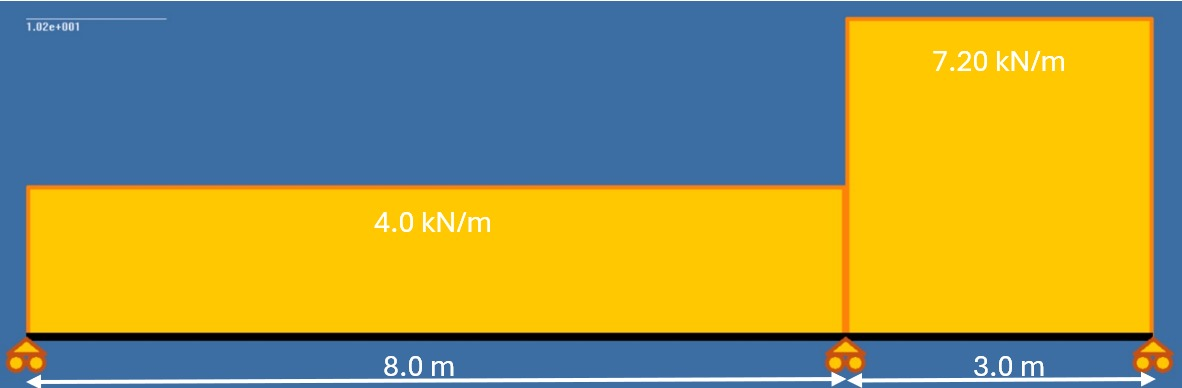
\includegraphics[width=0.92\textwidth]{figuras/xvigas_nervio2_cargas.jpeg}
    \caption{Modelo y cargas lineales del segundo nervio en Xvigas.}
    \label{fig:xvigas-cargas}
\end{figure}

\begin{figure}[H]
    \centering
    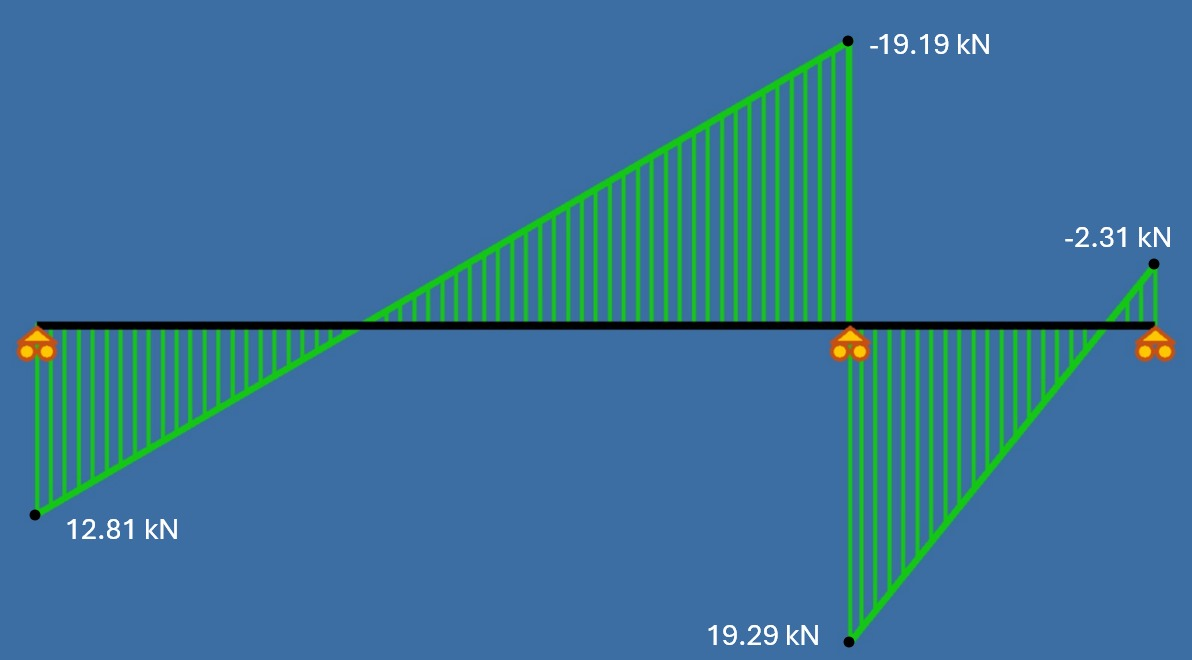
\includegraphics[width=0.92\textwidth]{figuras/xvigas_nervio2_cortante.jpeg}
    \caption{Diagrama de fuerza cortante del segundo nervio obtenido en Xvigas.}
    \label{fig:xvigas-cortante}
\end{figure}

\begin{figure}[H]
    \centering
    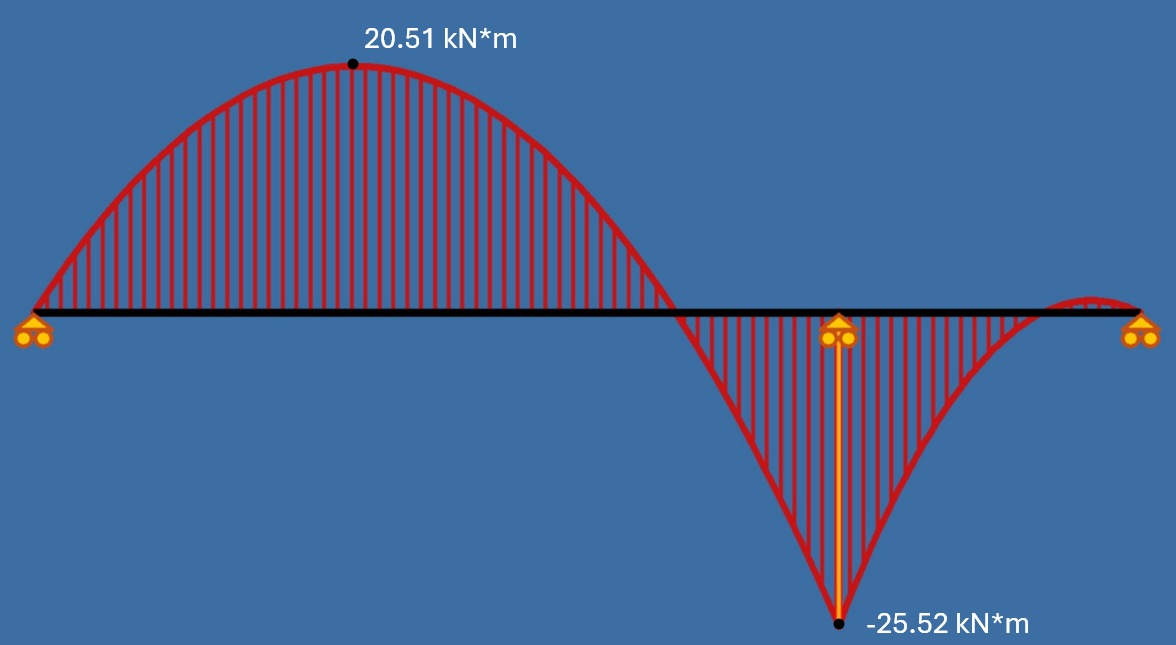
\includegraphics[width=0.92\textwidth]{figuras/xvigas_nervio2_momento.jpeg}
    \caption{Diagrama de momento flector del segundo nervio obtenido en Xvigas.}
    \label{fig:xvigas-momento}
\end{figure}

\section{Preselección del perfil de acero del nervio}
\label{sec:seleccion-perfil}

Para la preselección se adopta el mayor moment de los dos nervios estudiados, ya que no existe una diferencia drastica entre la magnitud de estos dos: $M_u=-25{,}52$ kN·m en el apoyo B del segundo nervio. 
\subsection{Conversión del momento y módulo resistente requerido}

La base de datos de perfiles está expresada en unidades inglesas por lo que se hace una conversión a este sistema. Con $1$ kN·m $=8{,}8507$ kip·in:

\begin{equation*}
|M_u|=25{,}52\times 8{,}8507=225{,}87\ \text{kip·in}
\end{equation*}

Para esta comparación preliminar se adopta acero ASTM A572 Grado 50, con $F_y=50$ ksi. El módulo resistente elástico requerido alrededor del eje fuerte se estima como:

\begin{equation*}
S_{\mathrm{req}}=\frac{|M_u|}{F_y}=\frac{225{,}87\ \text{kip·in}}{50\ \text{kip/in}^2}=4{,}52\ \text{in}^3
\end{equation*}

Se comparan secciones transversales tipo C y MC, excluyendo perfiles PHR C. Realizando un flitro inicial se obtienen los siguientes resultados.

\begin{table}[H]
    \centering
    \small
    \begin{tabular}{>{\raggedright\arraybackslash}p{2.4cm} c c c c >{\raggedright\arraybackslash}p{2.7cm}}
        \toprule
        Perfil & Altura (cm) & Peso (kg/m) & $S_x$ (in$^3$) & Reserva sobre $S_{\mathrm{req}}$ & Evaluación preliminar \\
        \midrule
        C6X8.2 & 15,24 & 12,20 & 4,35 & $-3,71\%$ & No cumple \\
        MC8X8.5 & 20,32 & 12,65 & 5,82 & $28,83\%$ & Seleccionado \\
        C7X9.8 & 17,78 & 14,58 & 6,07 & $34,37\%$ & Cumple; mayor peso \\
        MC10X6.5 & 25,40 & 9,67 & 4,59 & $1,61\%$ & Cumple ajustado; descartado por altura \\
        \bottomrule
    \end{tabular}
    \caption{Comparación preliminar de perfiles frente al módulo resistente requerido.}
    \label{tab:perfiles-preseleccion}
\end{table}

El perfil C6X8.2 no alcanza el módulo requerido para el momento gobernante. El MC10X6.5 apenas lo supera y se descarta por su altura de 25,40 cm, que incrementaría el peralte visible del nervio. El C7X9.8 ofrece mayor reserva, pero pesa 1,93 kg/m más que el MC8X8.5. Se preselecciona el MC8X8.5 por cumplir con una reserva de 28,83\% y mantener un peso moderado frente al C7X9.8. Además, se propone mantener una sección común para los nervios por criterio de constructibilidad.

La sección preseleccionada es MC8X8.5. Según la ficha consultada, tiene un área transversal de $2{,}5$ in$^2$, una masa lineal de $12{,}65$ kg/m, una altura total de $20{,}32$ cm y módulos resistentes elásticos $S_{\mathrm{bottom}}=S_{\mathrm{top}}=5{,}82$ in$^3$.

\begin{figure}[H]
    \centering
    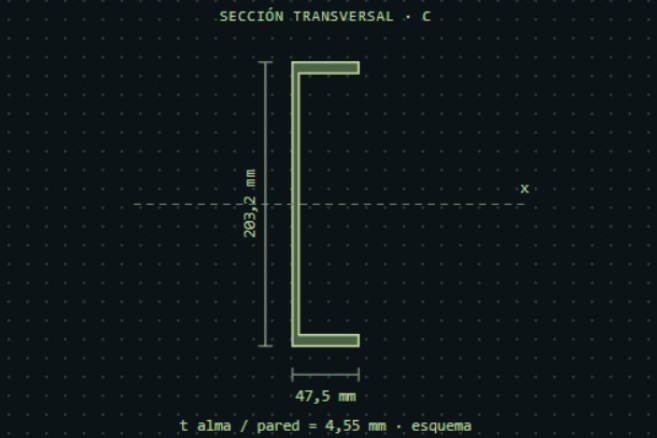
\includegraphics[width=0.72\textwidth]{figuras/seccion_perfil_mc8x8_5.png}
    \caption{Sección transversal del perfil MC8X8.5 preseleccionado.}
    \label{fig:seccion-perfil}
\end{figure}


\section{Nota}

Se utilizaron herramientas de inteligencia artificial como Codex y Claude para la elaboración del informe con la mayoría de graficas presentadas. Tanto el contenido del texto como el procedimiento, analisis y codigos empleados fueron elaboración propia.

\end{document}
